% Fused attention at two levels of abstraction: CUDA C++ and cuTile
% CS-6023 course project, OP2. Final report.
%
% Structure: problem statement, the mathematics used, the basic kernel idea, what was changed to make
% the kernels faster, comparisons and data, then references and source code.
%
% Build:  pdflatex report.tex      (run twice; pgfplots needs two passes)
%         or: tectonic report.tex
%
% Every number comes from results/benchmarks.csv or profiles/. Nothing is quoted from a datasheet.

\documentclass[10pt,a4paper]{article}

\usepackage[margin=1.45cm]{geometry}
\usepackage[T1]{fontenc}
\usepackage{newtxtext,newtxmath}      % Times-like body and matching maths
\usepackage{microtype}                % better spacing, fewer overfull boxes
\usepackage{booktabs}
\usepackage{pgfplots}
\pgfplotsset{compat=1.18}
\usepackage{siunitx}
\usepackage{amsmath}   % newtxmath already supplies \mathbb
\usepackage{caption}
\captionsetup{font=small,labelfont=bf,skip=3pt}
\usepackage{titlesec}
\usepackage{float}
\usepackage[hidelinks]{hyperref}

\titlespacing*{\section}{0pt}{5pt}{2pt}
\titleformat{\section}{\normalfont\large\bfseries}{\thesection}{0.6em}{}
\titleformat{\subsection}{\normalfont\normalsize\bfseries}{\thesubsection}{0.5em}{}
\titlespacing*{\subsection}{0pt}{4pt}{1pt}
\setlength{\parindent}{0pt}
\setlength{\parskip}{1.4pt}
\pagestyle{empty}

\newcommand{\cuda}{\textsc{cuda}}
\newcommand{\ctile}{\textsc{cuTile}}

\begin{document}

\begin{center}
{\LARGE\bfseries Fused Attention at Two Levels of Abstraction}\\[3pt]
{\large One operator written by hand and by compiler, then measured}\\[7pt]
Balla Surya Harshith \quad CS23B010 \quad CS-6023 GPU Programming\\
Mentor: Pravin Jagtap \quad 7 November 2026
\end{center}

\vspace{-6pt}
\section*{Summary}
I write the same fused attention forward pass twice on one consumer GPU. The first version uses CUDA
C++ at thread level. The second uses cuTile at tile level. Both are exact. Both pass an fp64 oracle at
every size and both masks, and they agree with each other to $2.5\times10^{-4}$. I then rewrite the
CUDA kernel so that its score tile, its softmax state and its accumulator stay in registers, and
measure what that change is worth. It reaches \textbf{107\%} of a ceiling I measured myself, is
\textbf{3.3$\times$} faster than the kernel it replaces, and is \textbf{4.5$\times$} faster than the
compiler's at $N{=}2048$. It wins five of the eight configurations, including every causal one, where
it is also faster than PyTorch SDPA. The cause is measured, not assumed: tensor-pipe utilisation rises
from 13.2\% to 42.2\%, against SDPA's 45.1\%, while the kernel moves one third of SDPA's DRAM traffic.

\section{Problem statement}

Attention is the operation inside a transformer that lets each position look at every other position.
For one head it is
\begin{equation}
O = \operatorname{softmax}\!\left(\frac{QK^{\top}}{\sqrt{D}} + M\right)V,
\qquad Q,K,V,O \in \mathbb{R}^{N\times D},
\label{eq:attn}
\end{equation}
with $N$ the sequence length, $D$ the head width, and $M$ a mask. This project uses
$B{=}1$ batch, $H{=}8$ heads and $D{=}64$.

The naive form materialises the $N\times N$ score matrix in global memory. At $N{=}2048$ and eight
heads that matrix is \SI{134}{MB} in fp32. It must be written, read, and written again for the second
product, so the operation becomes memory-bound and gives the tensor cores nothing to do. The measured
effect is in \S\ref{sec:data}: the materialised version reaches an effective \SI{31}{GB/s} against
\SI{170}{GB/s} available.

The task is therefore to \emph{fuse} the three stages into one kernel, so that the score matrix never
leaves the chip. Fusing forces two consequences that shape all the code that follows. First, the
softmax cannot see the whole row at once, so it must run in a streaming form. Second, the per-row
rescale that streaming implies must be applied to a live accumulator, and where that accumulator lives
is the single most important decision in the project (\S\ref{sec:faster}).

The brief asks for the operator at both levels of abstraction, then a written comparison across
development velocity, control and tunability, portability, achieved performance and debuggability.
Those five axes are answered in Table~\ref{tab:axes}.

\section{The mathematics used}

\paragraph{Softmax, exactly.} For row $i$ with logits $s_{ij}$,
$\operatorname{softmax}(s)_{ij} = \exp(s_{ij} - m_i) / \sum_j \exp(s_{ij} - m_i)$, where
$m_i = \max_j s_{ij}$. Subtracting the row maximum changes nothing mathematically. It prevents
overflow, because the largest exponent becomes zero.

\paragraph{Online softmax.} A streaming kernel sees one key tile at a time. It keeps a running maximum
$m$, a running normaliser $\ell$, and a running unnormalised output $\mathrm{acc}$. When a new tile
arrives, the tile maximum is $m_{\text{new}}$, and
\begin{equation}
\alpha = \exp\!\left(m_{\text{old}} - m_{\text{new}}\right),\quad
\ell \leftarrow \alpha\,\ell + \sum_j e^{\,s_j - m_{\text{new}}},\quad
\mathrm{acc} \leftarrow \alpha\,\mathrm{acc} + P V .
\label{eq:online}
\end{equation}
The factor $\alpha$ is applied exactly once per tile, before the accumulate. This recurrence gives the
same answer as the two-pass form, in one pass, with the row state bounded in size.

\paragraph{One exponential per element.} Both kernels work in base two. The scale is folded into the
QK product as $\log_2 e/\sqrt{D}$, so the softmax needs \texttt{exp2} only. The ablation that removed
\texttt{exp2} entirely changed the time by 0.0\% to 0.9\%, which shows the exponential is not the
bottleneck.

\paragraph{Masks.} Two are applied element-wise. A tail mask sets every key at or past $N$ to a finite
sentinel, because $-\infty$ would make $\alpha$ a NaN. A causal mask keeps only keys with
$\mathit{key} \le \mathit{query}$. Interior tiles need neither, which is what \S\ref{sec:faster}
exploits.

\paragraph{Precision rules.} Scores, the softmax state and the accumulator are fp32. Only the two
matmul inputs are fp16. This is a correctness rule, not a tuning choice: fp16 accumulation overflows
on these inputs, and the materialised baseline demonstrates it at a $\times100$ stress scale.

\paragraph{Cost.} The operation is $4N^2D$ FLOPs per head, so \SI{8.59}{GFLOP} at $N{=}2048$. Fused
traffic is $4ND$ halves per head in and out, \SI{8.4}{MB} in total, so the arithmetic intensity is
$\SI{1024}{FLOP/byte}$. Against a ridge point of 71 the fused form is compute-oriented, and the
materialised form is bandwidth-oriented at \SI{411}{MB}.

\section{The basic kernel idea}

Both kernels tile the problem the same way. A block owns 64 query rows. It walks the key dimension in
tiles of 64, and for each tile it does four things: compute the score tile $S = QK^{\top}$, mask it,
update the running softmax state, and accumulate $P V$. Q stays resident, K and V stream.

\begin{table}[H]
\centering\small
\caption{The same operator at two levels of abstraction. Resource figures come from
\texttt{cuobjdump -res-usage}; occupancy from \texttt{cudaOccupancyMaxActiveBlocksPerMultiprocessor},
which needs no profiler counter.}
\label{tab:impl}
\begin{tabular}{@{}llll@{}}
\toprule
 & \cuda{} v1 & \cuda{} v2 (shipped) & \ctile{} \\
\midrule
Work mapping & 128 threads; 16 query rows per warp & same & one block per 64-row tile; no thread index \\
Matrix multiply & \texttt{wmma} m16n16k16 & \texttt{mma.sync} m16n8k16 & \texttt{ct.mma} on whole tiles \\
Fragments & \texttt{wmma} load/store & \texttt{ldmatrix}, V transposed & chosen by the compiler \\
Accumulator & shared memory & \textbf{registers} & registers, compiler's choice \\
Softmax & scalar, 2 lanes per row & per lane, quad shuffle & \texttt{ct.max}, \texttt{ct.exp2}, \texttt{ct.sum} \\
Async copy & none & \texttt{cp.async}, double buffered & compiler's choice (\texttt{LDGSTS}) \\
Registers & 56 & 140 & 255 \\
Shared memory & 72192 B & 46080 B & 48 KB \\
Blocks per SM & 1 & \textbf{2} & 2 \\
Source & 138 code lines & 191 code lines & 118 code lines \\
\bottomrule
\end{tabular}
\end{table}

The compiler version needs 118 lines and contains no thread index, no stride, no barrier and no staging
decision. The hand-written versions need those decisions, which is the trade the brief asks us to
measure.

\section{What was done to make the kernels faster}\label{sec:faster}

Each change below was made because a measurement named the bottleneck. Table~\ref{tab:steps} records
what each was worth and how it was checked.

\begin{table}[H]
\centering\small
\caption{Optimisation ladder. Every row was verified before it was believed: correctness against the
fp64 oracle, then timing. Figures are p50 at the size named in the row.}
\label{tab:steps}
\begin{tabular}{@{}p{3.5cm}p{4.4cm}rrl@{}}
\toprule
change & bottleneck it targets & before & after & check \\
\midrule
Pad shared strides to 68/72, interleave lane columns & 32-way bank conflict: every lane hit one bank &
\SI{9146}{\micro\second} & \SI{3594}{\micro\second} & error unchanged to the last digit \\
Remove a per-call device synchronise & unfair timer, not the kernel & \SI{107.5}{\micro\second} &
\SI{42.0}{\micro\second} & events agree with wall clock within 1\% \\
Stage K and V with 16-byte loads & exposed DRAM latency from scalar 2-byte loads &
\SI{3207.8}{\micro\second} & \SI{2091.4}{\micro\second} & \texttt{LDG.E.128} replaces 19 scalar sites \\
Keep S, P and the accumulator in registers & shared-memory round trip per tile, and occupancy &
\SI{2172.7}{\micro\second} & \SI{664.2}{\micro\second} & 0 spills; oracle identical; 2 blocks/SM \\
Mask only diagonal and tail tiles & compare and select on every tile & --- & --- & branch is uniform \\
\bottomrule
\end{tabular}
\end{table}

\paragraph{The decision that mattered.} A WMMA accumulator fragment has a layout that the WMMA API does
not expose, so a per-row rescale is not expressible while the accumulator stays in registers. The first
kernel therefore put the accumulator in shared memory. That cost a round trip per tile, and at
72192~B it allowed one block per SM, which is \SI{8.3}{\%} occupancy. Moving to
\texttt{mma.sync.m16n8k16}, whose fragment map I verified on this GPU with a probe, removed the
restriction. The score tile, the probabilities and the accumulator then live in registers, shared
memory falls to 46080~B, and two blocks fit per SM. Occupancy doubles and tensor-pipe utilisation triples.

\paragraph{Two fixes with no measurable effect, kept for honesty.} The exponential is not the
bottleneck (0.0\% to 0.9\%). Hoisting a predicate cut registers from 63 to 56 but moved the time inside
noise. Both are recorded because a clean table is less useful than an accurate one.

\section{Comparisons and data}\label{sec:data}

Five implementations share one harness, one oracle and one timer. Each configuration is timed six
times, and the six p50 values are averaged. The spread of the mean is 0.0 to \SI{2.8}{\micro\second}
for the GPU kernels.

\begin{table}[H]
\centering\small
\caption{p50 latency, \textmu s, mean of six repetitions, at least one second of GPU work per
repetition with the L2 flushed outside the timed window. \emph{Bold} marks the best model in the row.}
\label{tab:perf}
\begin{tabular}{@{}rrrrrrl@{}}
\toprule
$N$ & causal & \cuda{} v1 & \cuda{} v2 & \ctile{} & unfused & SDPA \\
\midrule
256 & no & 49.2 & \textbf{18.6} & 42.0 & 807.5 & 19.5 \\
256 & yes & 49.2 & \textbf{19.5} & 21.5 & 1032.1 & 20.5 \\
512 & no & 157.7 & 52.1 & 150.5 & 1020.5 & \textbf{49.2} \\
512 & yes & 122.9 & \textbf{41.0} & 53.1 & 1269.6 & 52.2 \\
1024 & no & 575.0 & 176.1 & 622.4 & 3562.1 & \textbf{163.8} \\
1024 & yes & 359.4 & \textbf{109.6} & 134.7 & 3961.7 & 129.0 \\
2048 & no & 2172.7 & 664.2 & 2991.2 & 13314.9 & \textbf{616.6} \\
2048 & yes & 1197.6 & \textbf{364.5} & 447.9 & 15097.9 & 397.0 \\
\bottomrule
\end{tabular}
\end{table}

\begin{figure}[H]
\centering
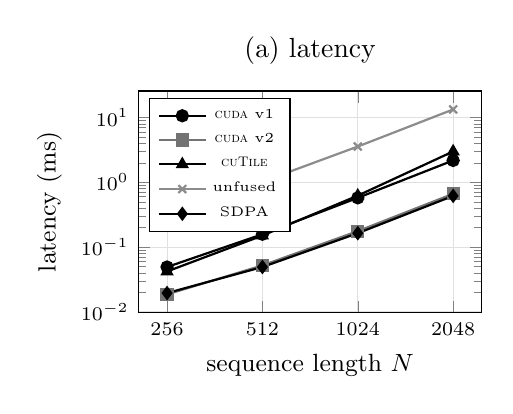
\begin{tikzpicture}
\begin{axis}[
  width=0.49\textwidth, height=4.4cm,
  xlabel={sequence length $N$}, ylabel={latency (ms)},
  xmode=log, log basis x=2, ymode=log,
  xtick={256,512,1024,2048}, xticklabels={256,512,1024,2048},
  legend pos=north west, legend style={font=\tiny},
  grid=major, grid style={black!12}, tick label style={font=\scriptsize},
  label style={font=\small}, title={(a) latency},
]
\addplot[mark=*, thick] coordinates {(256,0.0492) (512,0.1577) (1024,0.5750) (2048,2.1727)};
\addplot[mark=square*, thick, black!55] coordinates {(256,0.0186) (512,0.0521) (1024,0.1761) (2048,0.6642)};
\addplot[mark=triangle*, thick] coordinates {(256,0.0420) (512,0.1505) (1024,0.6224) (2048,2.9912)};
\addplot[mark=x, thick, black!45] coordinates {(256,0.8075) (512,1.0205) (1024,3.5621) (2048,13.3149)};
\addplot[mark=diamond*, thick] coordinates {(256,0.0195) (512,0.0492) (1024,0.1638) (2048,0.6166)};
\legend{\cuda{} v1, \cuda{} v2, \ctile, unfused, SDPA}
\end{axis}
\end{tikzpicture}\hfill
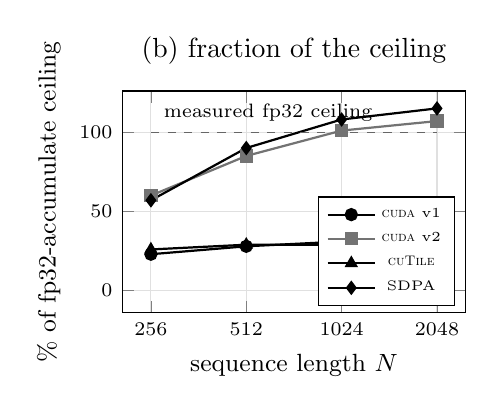
\begin{tikzpicture}
\begin{axis}[
  width=0.49\textwidth, height=4.4cm,
  xlabel={sequence length $N$}, ylabel={\% of fp32-accumulate ceiling},
  xmode=log, log basis x=2,
  xtick={256,512,1024,2048}, xticklabels={256,512,1024,2048},
  ymin=-14, ymax=126, legend pos=south east, legend style={font=\tiny},
  grid=major, grid style={black!12}, tick label style={font=\scriptsize},
  label style={font=\small}, title={(b) fraction of the ceiling},
]
\addplot[mark=*, thick] coordinates {(256,23) (512,28) (1024,31) (2048,33)};
\addplot[mark=square*, thick, black!55] coordinates {(256,60) (512,85) (1024,101) (2048,107)};
\addplot[mark=triangle*, thick] coordinates {(256,26) (512,29) (1024,29) (2048,24)};
\addplot[mark=diamond*, thick] coordinates {(256,57) (512,90) (1024,108) (2048,115)};
\draw[dashed, black!60] (axis cs:256,100) -- (axis cs:2048,100);
\node[font=\scriptsize, anchor=south west] at (axis cs:262,101) {measured fp32 ceiling};
\legend{\cuda{} v1, \cuda{} v2, \ctile, SDPA}
\end{axis}
\end{tikzpicture}
\caption{(a) Latency against sequence length. The fused kernels are one to two orders of magnitude
below the materialised baseline at the largest size. (b) The same data as a fraction of the
\SI{12.1}{TFLOP/s} fp32-accumulate ceiling. SDPA crosses that line, so it is not issuing the
instruction the line describes.}
\label{fig:perf}
\end{figure}

\paragraph{Correctness.} The fp64 oracle passes at every size and both masks. Both kernels give the same
$\max|o-o_{\text{ref}}|$ to the last digit, which is the strongest available evidence, because a shared
bug across two very different layouts is implausible. Six cases are representative: $N{=}1$ gives
\SI{0.0}{}, $N{=}65$ gives $4.48\times10^{-4}$, $N{=}1000$ gives $1.32\times10^{-4}$, and $N{=}2048$
gives $7.91\times10^{-5}$ non-causal and $9.73\times10^{-4}$ causal, all against an allowance of
$5\times10^{-3}\max|o_{\text{ref}}|$. In addition, 38 closed-form checks use mathematics rather than
the oracle: with $V{=}\mathbf{1}$ the output must be exactly $\mathbf{1}$ (it is, to 0.0), with
$Q{=}\mathbf{0}$ it must be the running mean of $V$, and a one-hot key must return that row of $V$. A
further 19 checks cover determinism, tile boundaries 63/64/127/128/4095/4097, and fp16 overflow.

\paragraph{Where the time now goes.} The counters explain the ordering better than the source does.

\begin{table}[H]
\centering\small
\caption{Measured DRAM traffic and utilisation at $N{=}2048$, one profiled launch per row
(\texttt{ncu} with \texttt{dram\_\_bytes\_*}, \texttt{sm\_\_warps\_active} and the tensor-pipe cycle
counters). The ideal fused traffic is \SI{8.4}{MB} in total.}
\label{tab:dram}
\begin{tabular}{@{}lrrrrr@{}}
\toprule
kernel & causal & DRAM read & DRAM write & warps active & tensor pipe \\
\midrule
\cuda{} v1 & no & 6.33 MB & 1.77 MB & 8.3\% & 13.2\% \\
\cuda{} v2 & no & 6.31 MB & 1.73 MB & \textbf{16.3\%} & \textbf{42.2\%} \\
\cuda{} v1 & yes & 6.36 MB & 2.28 MB & 8.3\% & 12.1\% \\
\cuda{} v2 & yes & 6.31 MB & 1.73 MB & \textbf{16.5\%} & \textbf{39.9\%} \\
\ctile{} & no & 57.24 MB & \textbf{321.93 MB} & 16.5\% & 13.8\% \\
\ctile{} & yes & 6.35 MB & 1.77 MB & 16.1\% & 31.0\% \\
SDPA & no & 6.87 MB & 3.06 MB & 15.9\% & 45.1\% \\
\bottomrule
\end{tabular}
\end{table}

Two findings come from this table and neither was visible in the source. First, \textbf{the compiler's
non-causal build is not fused}: it writes \SI{322}{MB}, about 2.8 times one $N\times N$ fp32 matrix,
while the same source compiled for the causal case writes \SI{1.77}{MB}. One compilation stays on chip
and the other leaks, and only a counter separates them. Second, \textbf{the gap to SDPA was tensor-pipe
utilisation and nothing else}: 45.1\% against 13.2\%, which is the 3.42$\times$ latency ratio almost
exactly. Raising it to 42.2\% is what closed that gap to 1.08$\times$.

\paragraph{The five axes.}

\begin{table}[H]
\centering\small
\caption{The brief's five axes, each answered by an observation rather than an opinion.}
\label{tab:axes}
\begin{tabular}{@{}p{2.6cm}p{13.4cm}@{}}
\toprule
axis & evidence \\
\midrule
Development velocity & 118 code lines of cuTile against 138 and 191 for the two CUDA versions. The CUDA
kernels needed five measured fixes; cuTile needed one loop bound. cuTile's advantage is not typing
speed, it is the bug classes that cannot occur. \\
Control and tunability & I must choose the fragment mapping, the shared stride and padding, the barrier
placement and the staging width. cuTile exposes tile shape, latency hints and per-architecture policy,
and decides storage itself. The accumulator is the sharp case: I am forced into shared memory with
WMMA, and the compiler is not. \\
Portability & Argued, not measured: one GPU was available. My kernel hard-codes 46080~B for sm\_86;
cuTile carries architecture policy and emits architecture-appropriate copies. \\
Performance & The shipped kernel is 4.5$\times$ faster than cuTile at $N{=}2048$ non-causal and
1.23$\times$ faster causal, at 107\% and 97\% of a measured ceiling. SDPA remains 1.08$\times$ faster
non-causal, and it exceeds that ceiling, so part of its lead is a narrower accumulate than our rule
allows. \\
Debuggability & SASS, \texttt{ptxas} resource reports and the occupancy API are available to both, and
they are what found the defects. cuTile gives up the source-to-instruction correspondence: I can map my
assembly to my lines, but not the compiler's. \\
\bottomrule
\end{tabular}
\end{table}

\section{Conclusion and recommendation}

\textbf{Start in cuTile, and expect to finish in CUDA.} The tile version was correct, and it cost 118
lines with no thread index, no stride and no barrier. It is the right way to find out whether the
operator matters at all.

\textbf{Decide with counters, not with line counts.} The same 118 lines produced one kernel that stays
on chip and one that writes \SI{322}{MB} to DRAM. The causal build, which does not leak, still reached
only 31\% of the tensor pipe against SDPA's 45\%.

\textbf{Take the control back for one specific reason: where the accumulator lives.} That is the choice
the tile source cannot express, and here it was worth 3.3$\times$: from 33\% to 107\% of the measured
ceiling. When a profile says the remaining gap is a register-versus-shared-memory decision, the
hand-written kernel is not a preference. Before that point it is a way to lose two weeks.

\section*{Limitations}
One GPU (sm\_86, 4 GB, no TMA, no clusters, no FP8), so portability is argued rather than measured.
Forward pass only. GPU counters were unavailable until the final hours, so Table~\ref{tab:dram} holds
the only profiled data here and the baseline's traffic is still inferred. The fused-versus-unfused ratio
is an upper bound, because the baseline casts to fp32 to avoid fp16 overflow. The fp32 softmax-state
rule costs throughput by construction: the same tensor cores accept a narrower accumulate at twice the
rate, which is where SDPA's remaining lead comes from.

\begin{thebibliography}{9}\footnotesize
\setlength{\itemsep}{1pt}\setlength{\parskip}{0pt}
\bibitem{fa1} T.~Dao, D.~Y.~Fu, S.~Ermon, A.~Rudra, C.~R\'e. \emph{FlashAttention: Fast and
Memory-Efficient Exact Attention with IO-Awareness}. NeurIPS 2022. arXiv:2205.14135.
\bibitem{fa2} T.~Dao. \emph{FlashAttention-2: Faster Attention with Better Parallelism and Work
Partitioning}. arXiv:2307.08691, 2023.
\bibitem{online} M.~Milakov, N.~Gimelshein. \emph{Online normalizer calculation for softmax}.
arXiv:1805.02867, 2018.
\bibitem{ptx} NVIDIA. \emph{Parallel Thread Execution ISA}, \S9.7.16 --- \texttt{mma} and
\texttt{ldmatrix} fragment layouts. \url{https://docs.nvidia.com/cuda/parallel-thread-execution/}
\bibitem{cutile} NVIDIA. \emph{cuTile Python documentation}.
\url{https://docs.nvidia.com/cuda/cutile-python/}
\bibitem{ampere} NVIDIA. \emph{Ampere Tuning Guide}.
\url{https://docs.nvidia.com/cuda/ampere-tuning-guide/}
\end{thebibliography}

\section*{Source code}
\begin{tabular}{@{}ll@{}}
\texttt{kernels/cuda-fused-attn/flash\_v2.cu} & the shipped CUDA kernel: \texttt{mma.sync},
\texttt{ldmatrix}, \texttt{cp.async}, register-resident \\
\texttt{kernels/cutile-fused-attn/flash.py} & the tile-level kernel: the same fusion in tile vocabulary \\
\texttt{baseline/attn/unfused.py} & the materialised reference: cuBLAS, softmax, cuBLAS \\
\texttt{bench/bench.py} & oracle, three models, timing protocol, CSV \\
\texttt{bench/peak.cu} & the fp32 and fp16 tensor-core ceiling benchmark \\
\texttt{scripts/} & closed-form checks, protocol checks, the emulator, the profiler \\
\end{tabular}

\end{document}
